%%%%%%%%%%%%%%%%%%%% Documentación del sistema %%%%%%%%%%%%%%%%%%%%


\section{Documentación de sistema}

Documentación referida a los aspectos del análisis, diseño, implementación y prueba del \textit{software}, así como la implantación del mismo. En general, debe hacer referencia al sistema, ya que está orientada a los programadores que van a realizar el mantenimiento. Debe estar muy bien estructurada, desde lo más general a los más interno.   


\subsection{Especificación del sistema}

Esta sección debe describir el análisis y la especificación de requisitos. Cómo se descompone el problema en distintos subproblemas y los módulos asociados a cada uno de ellos, acompañados de su especificación. También debe incluir el plan de desarrollo del \textit{software}.  


\subsection{Módulos}

\begin{itemize}

	\item \textbf{Salas}: Este módulo se encarga del administrado tanto de las conexiones como de las salas que componen el escape room. Posee funciones para la carga de conexiones y salas; liberarlas de la memoria, obtener una sala por su ID, y obtener la sala inicial de la partida actual. Este módulo muestra en pantalla errores si no se pudieron cargar los datos de las salas y/o conexiones, o si poseen un formato incorrecto en alguno de sus campos.

	\item \textbf{UI (Interfaz de Usuario)}: Este módulo se centra en pedir información al usuario y mostrarla por pantalla. Posee funciones para la creación de menús, vaciar el buffer de entrada, esperar a que el usuario presione una tecla para continuar, elegir SÍ o NO, mostrar el logo del juego y otros elementos por pantalla; salir del juego, mostrar los menús de registro o inicio de sesión, y el menú principal (el módulo '\textbf{partida} usa sus funciones para crear el menú de juego); mostrar los datos de las estructuras cargadas por memoria dinámica con la opción de poner filtros (por ejemplo, para solo ver los objetos en la sala actual); mostrar las interfaces de las diferentes opciones del menú de juego y de salir del juego mostrando unos breves créditos con los miembros creadores del trabajo.

\end{itemize}


\subsection{Plan de prueba}

Debe describir todo el plan de pueba que se ha llevado a cabo. Se distinguen las pruebas realizadas a cada módulo y las pruebas de integración de los distintos módulos probándolo como un todo. Por último, también se debe incluir la descripción del plan de pruebas de aceptación.  


\subsubsection{Prueba de los módulos}

\begin{itemize}

	\item \textbf{Pruebas de ruta básica de ''salas\_get\_sala\_from\_id'' (José Miguel Pérez Tejero):}
	
		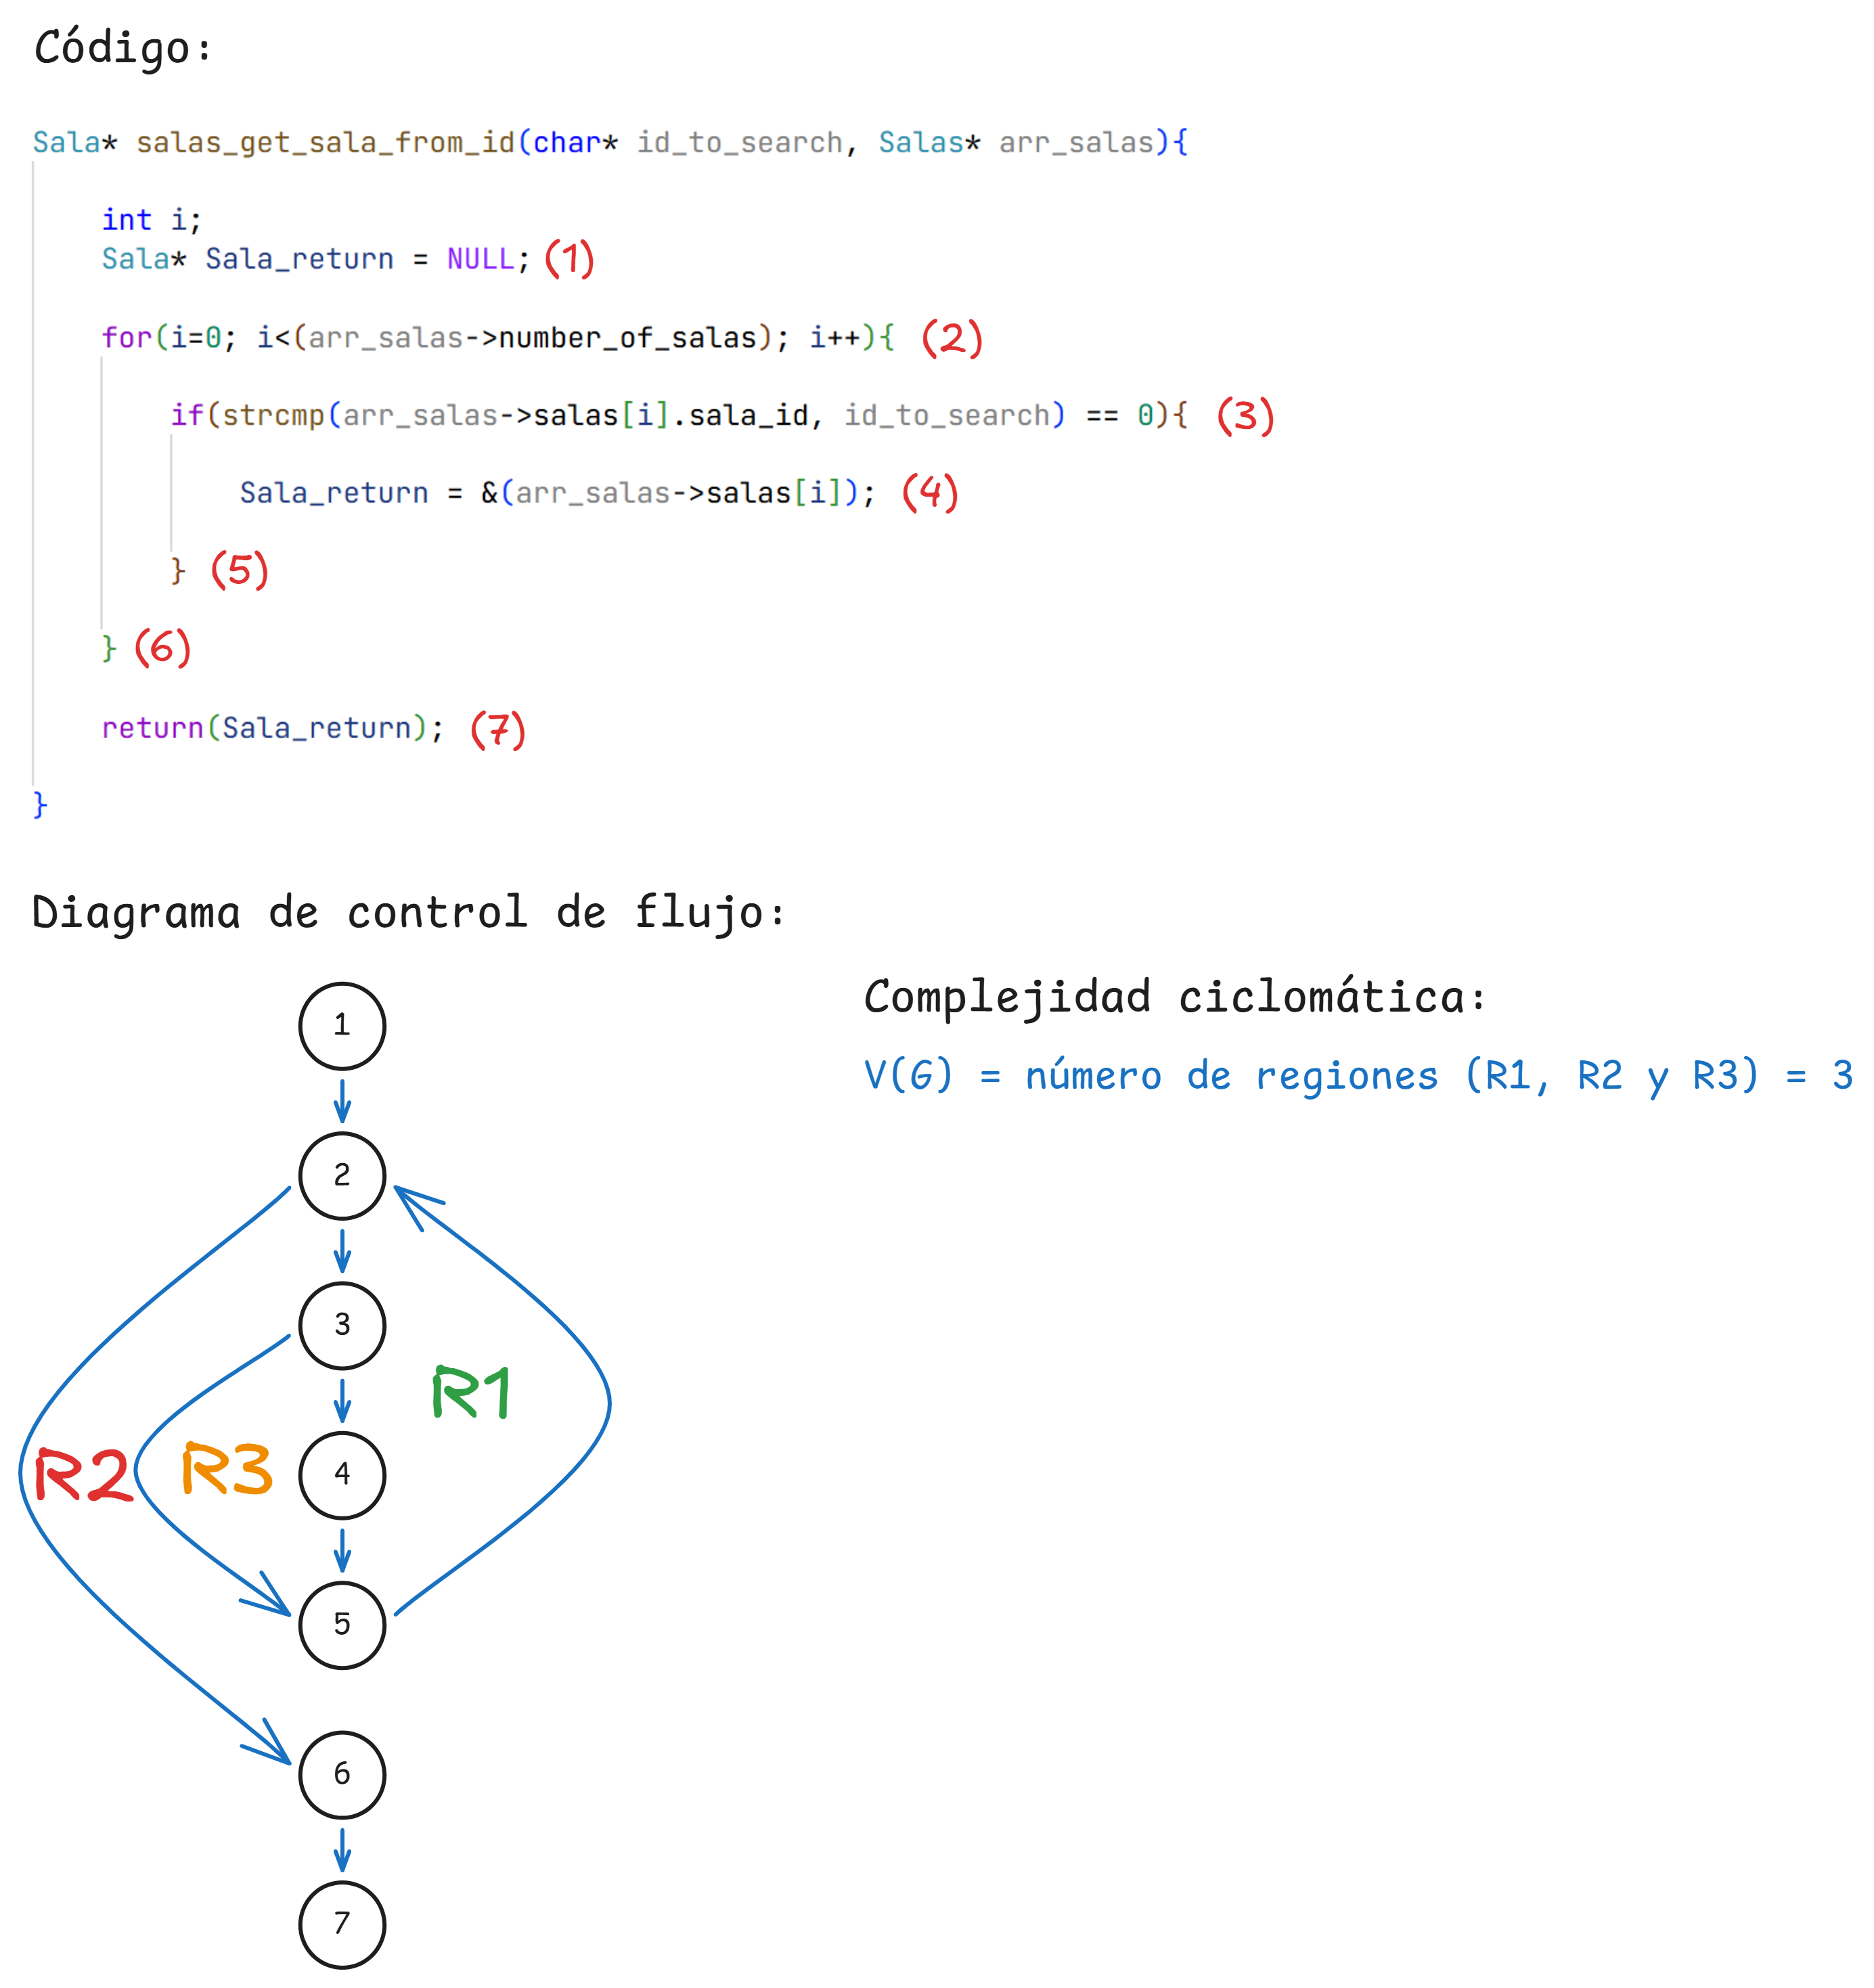
\includegraphics[width=1\textwidth]{Salas_get_salas_by_id_grafo.png} \bigskip

		\pagebreak

		\textbf{Casos de prueba:}

		\item \underline{Ruta 1 (1-2-6-7) (No entramos en el for):}
	
			Para llegar a un caso en el que no entremos al for, el número asociado al número de salas debe ser menor que 1.\\Así pues, un caso de prueba sería en el cual ''\verb|number_of_salas|'' es menor que 1.

		\item \underline{Ruta 2 (1-2-3-5-2-6-7) (Entramos en el for pero no entramos en el if):}

			Para entrar en esa ruta, no debe de haber ninguna sala que comparta el valor de ''\verb|id_to_search|'', y ''\verb|number_of_salas|'' debe ser mayor o igual que 1. \\
			También probaremos casos donde ''\verb|number_of_salas|'' supere al número real de salas.

		\item \underline{Ruta 3 (1-2-3-4-5-2-6-7) (Entramos en el for y en el if):}
		
			Aquí ''\verb|number_of_salas|'' será mayor o igual que 1, coincidirá con el número de salas, y habrá una sala mínima cuyo ID coincida con ''\verb|id_to_search|''. \\
			Así pues, diseñaremos casos de prueba que cumplan dichas condiciones.

\end{itemize}

\subsubsection{Prueba de integración}

Incluir toda la batería de pruebas realizadas. Pruebas de caja blanca y pruebas de caja negra.  


\subsubsection{ Plan de pruebas de aceptación}

Estas pruebas deben diseñarse con el usuario del sistema. Deben describir las pruebas que son necesarias pasar para que el sistema sea aceptado por el usuario final.  

\bigskip

Si en algún punto del documento se quiere hacer referencia a algún documento es necesario incluir la cita donde corresponda, podemos tomar como ejemplo \cite{Ejemplo3}. 